\section{Eksperimenti i analiza rezultata}
\label{sec:eksperimenti}

U ovom poglavlju detaljno se opisuje eksperimentalni postav, provedba eksperimenata te analiza i interpretacija dobivenih rezultata. Cilj je bio empirijski validirati predloženi hibridni model i usporediti ga s drugim pristupima.

\subsection{Postavke okruženja i testni podaci}
Svi eksperimenti provedeni su u programskom okruženju Python (verzija 3.x) na standardnom osobnom računalu. Za potrebe istraživanja generiran je sintetički skup podataka koji oponaša realističan projektni portfelj. U ovisnosti o eksperimentalnoj seriji, broj jedinstvenih projektnih aktivnosti varirao je od 10 do 100. Za svaku aktivnost definirani su sljedeći parametri unutar zadanih raspona:
\begin{itemize}
    \item \textbf{Trošak (\texttt{cost}):} Slučajna cjelobrojna vrijednost između 50 i 200.
    \item \textbf{ROI (\texttt{roi}):} Slučajna decimalna vrijednost između 1.0 i 3.0.
    \item \textbf{Procjene trajanja:}
    \begin{itemize}
        \item Optimistično: između 5 i 10 dana.
        \item Najvjerojatnije: između 10 i 20 dana.
        \item Pesimistično: između 20 i 40 dana.
    \end{itemize}
\end{itemize}
Ukupni raspoloživi budžet za portfelj (\texttt{BUDGET}) bio je skaliran u skladu sa složenošću problema.

\subsection{Eksperimentalni dizajn}
Kako bi se osigurala metodološka ispravnost i izbjegli proizvoljni zaključci, istraživanje je provedeno kroz dvo-fazni eksperimentalni proces:
\begin{itemize}
    \item \textbf{Faza 1: Analiza i kalibracija genetskog algoritma.} U prvoj fazi provedena je detaljna ablacijska studija kako bi se utvrdilo koji parametri genetskog algoritma daju najkvalitetnija i najstabilnija rješenja za reprezentativni tip problema (50 aktivnosti). Cilj je bio pronaći ``šampionsku'' konfiguraciju GA.
    \item \textbf{Faza 2: Usporedna analiza optimizacijskih modela.} U drugoj fazi, ``šampionska'' konfiguracija GA, dobivena u prvoj fazi, korištena je kao osnova za provođenje konačne usporedbe triju različitih optimizacijskih scenarija i evaluaciju glavnih hipoteza rada na problemima različite skale i restriktivnosti.
\end{itemize}

\subsubsection{Istraživačke hipoteze}
Na temelju teorijske podloge i postavljenih istraživačkih pitanja iz Uvoda, definirane su sljedeće tri glavne hipoteze koje će se provjeriti kroz eksperimente:

\begin{description}
    \item[H1 (Hipoteza o Skalabilnosti):] Povećanjem složenosti problema (broja aktivnosti), performanse modela temeljenog na nasumičnoj pretrazi (Random Search) će se značajno smanjiti u usporedbi s modelima temeljenim na genetskim algoritmima.
    \item[H2 (Hipoteza o Kompromisu):] Hibridni `GA+MC` model će, za razliku od klasičnog `GA (samo ROI)` modela, uspješno identificirati rješenja koja predstavljaju superioran kompromis između profitabilnosti (ROI) i rizika (trajanje projekta), posebno na problemima veće složenosti.
    \item[H3 (Hipoteza o Utjecaju Ograničenja):] Restriktivnost problema, specifično kroz promjenu raspoloživog budžeta, značajno utječe na performanse i stabilnost optimizacijskih modela, pri čemu se očekuje da će ekstremna ograničenja predstavljati najveći izazov za najsloženije modele.
\end{description}

\subsection{Eksperiment 1: Analiza parametara i kalibracija genetskog algoritma}

\textbf{Cilj:} Empirijski provjeriti utjecaj osnovnih genetskih operatora i parametara na performanse algoritma te odabrati optimalnu konfiguraciju za daljnje testiranje.

\textbf{Metodologija:} Provedena je ablacijska studija s pet različitih konfiguracija, gdje je svaka pokrenuta 10 puta (\texttt{RUNS = 10}) radi statističke pouzdanosti. Testirane konfiguracije su bile: \emph{Standardni GA}, \emph{Bez mutacije}, \emph{Bez križanja}, \emph{Više generacija} i \emph{Veća populacija}.

\textbf{Rezultati i diskusija:} Rezultati ablacijske studije prikazani su u Tablici~\ref{tab:ga_ablation} te grafički na Slici~\ref{fig:ga_ablation}.

\begin{table}[H]
    \centering
    \caption{Rezultati ablacijske studije za parametre GA.}
    \label{tab:ga_ablation}
    \begin{tabular}{|l|c|c|c|c|}
        \hline
        \textbf{Postavka} & \textbf{ROI\_mean} & \textbf{ROI\_std} & \textbf{Trajanje\_mean} & \textbf{Trajanje\_std} \\
        \hline
        Standardni GA & 28.985 & 1.543 & 199.216 & 10.691 \\
        Bez mutacije & 27.627 & 1.581 & 193.497 & 11.364 \\
        Bez križanja & 25.884 & 1.865 & 191.514 & 9.174 \\
        Više generacija & 31.183 & 0.928 & 205.026 & 13.649 \\
        \textbf{Veća populacija} & \textbf{31.683} & \textbf{0.720} & \textbf{213.694} & \textbf{5.574} \\
        \hline
    \end{tabular}
\end{table}

Analiza rezultata potvrđuje obje početne hipoteze. Uklanjanje križanja drastično smanjuje performanse, potvrđujući da je rekombinacija dobrih rješenja ključan mehanizam pretrage. Povećanje računalnih resursa, posebno kroz veću populaciju, dovodi do superiornih i statistički stabilnijih rješenja. Zanimljivo je primijetiti da konfiguracije s najvišim ROI-em rezultiraju i najdužim prosječnim trajanjem, što stvara prirodni kompromis (\emph{trade-off}) između profita i rizika, koji će biti predmet analize u sljedećem eksperimentu.

\begin{figure}[H]
    \centering
    \begin{subfigure}[b]{0.48\textwidth}
        \centering
        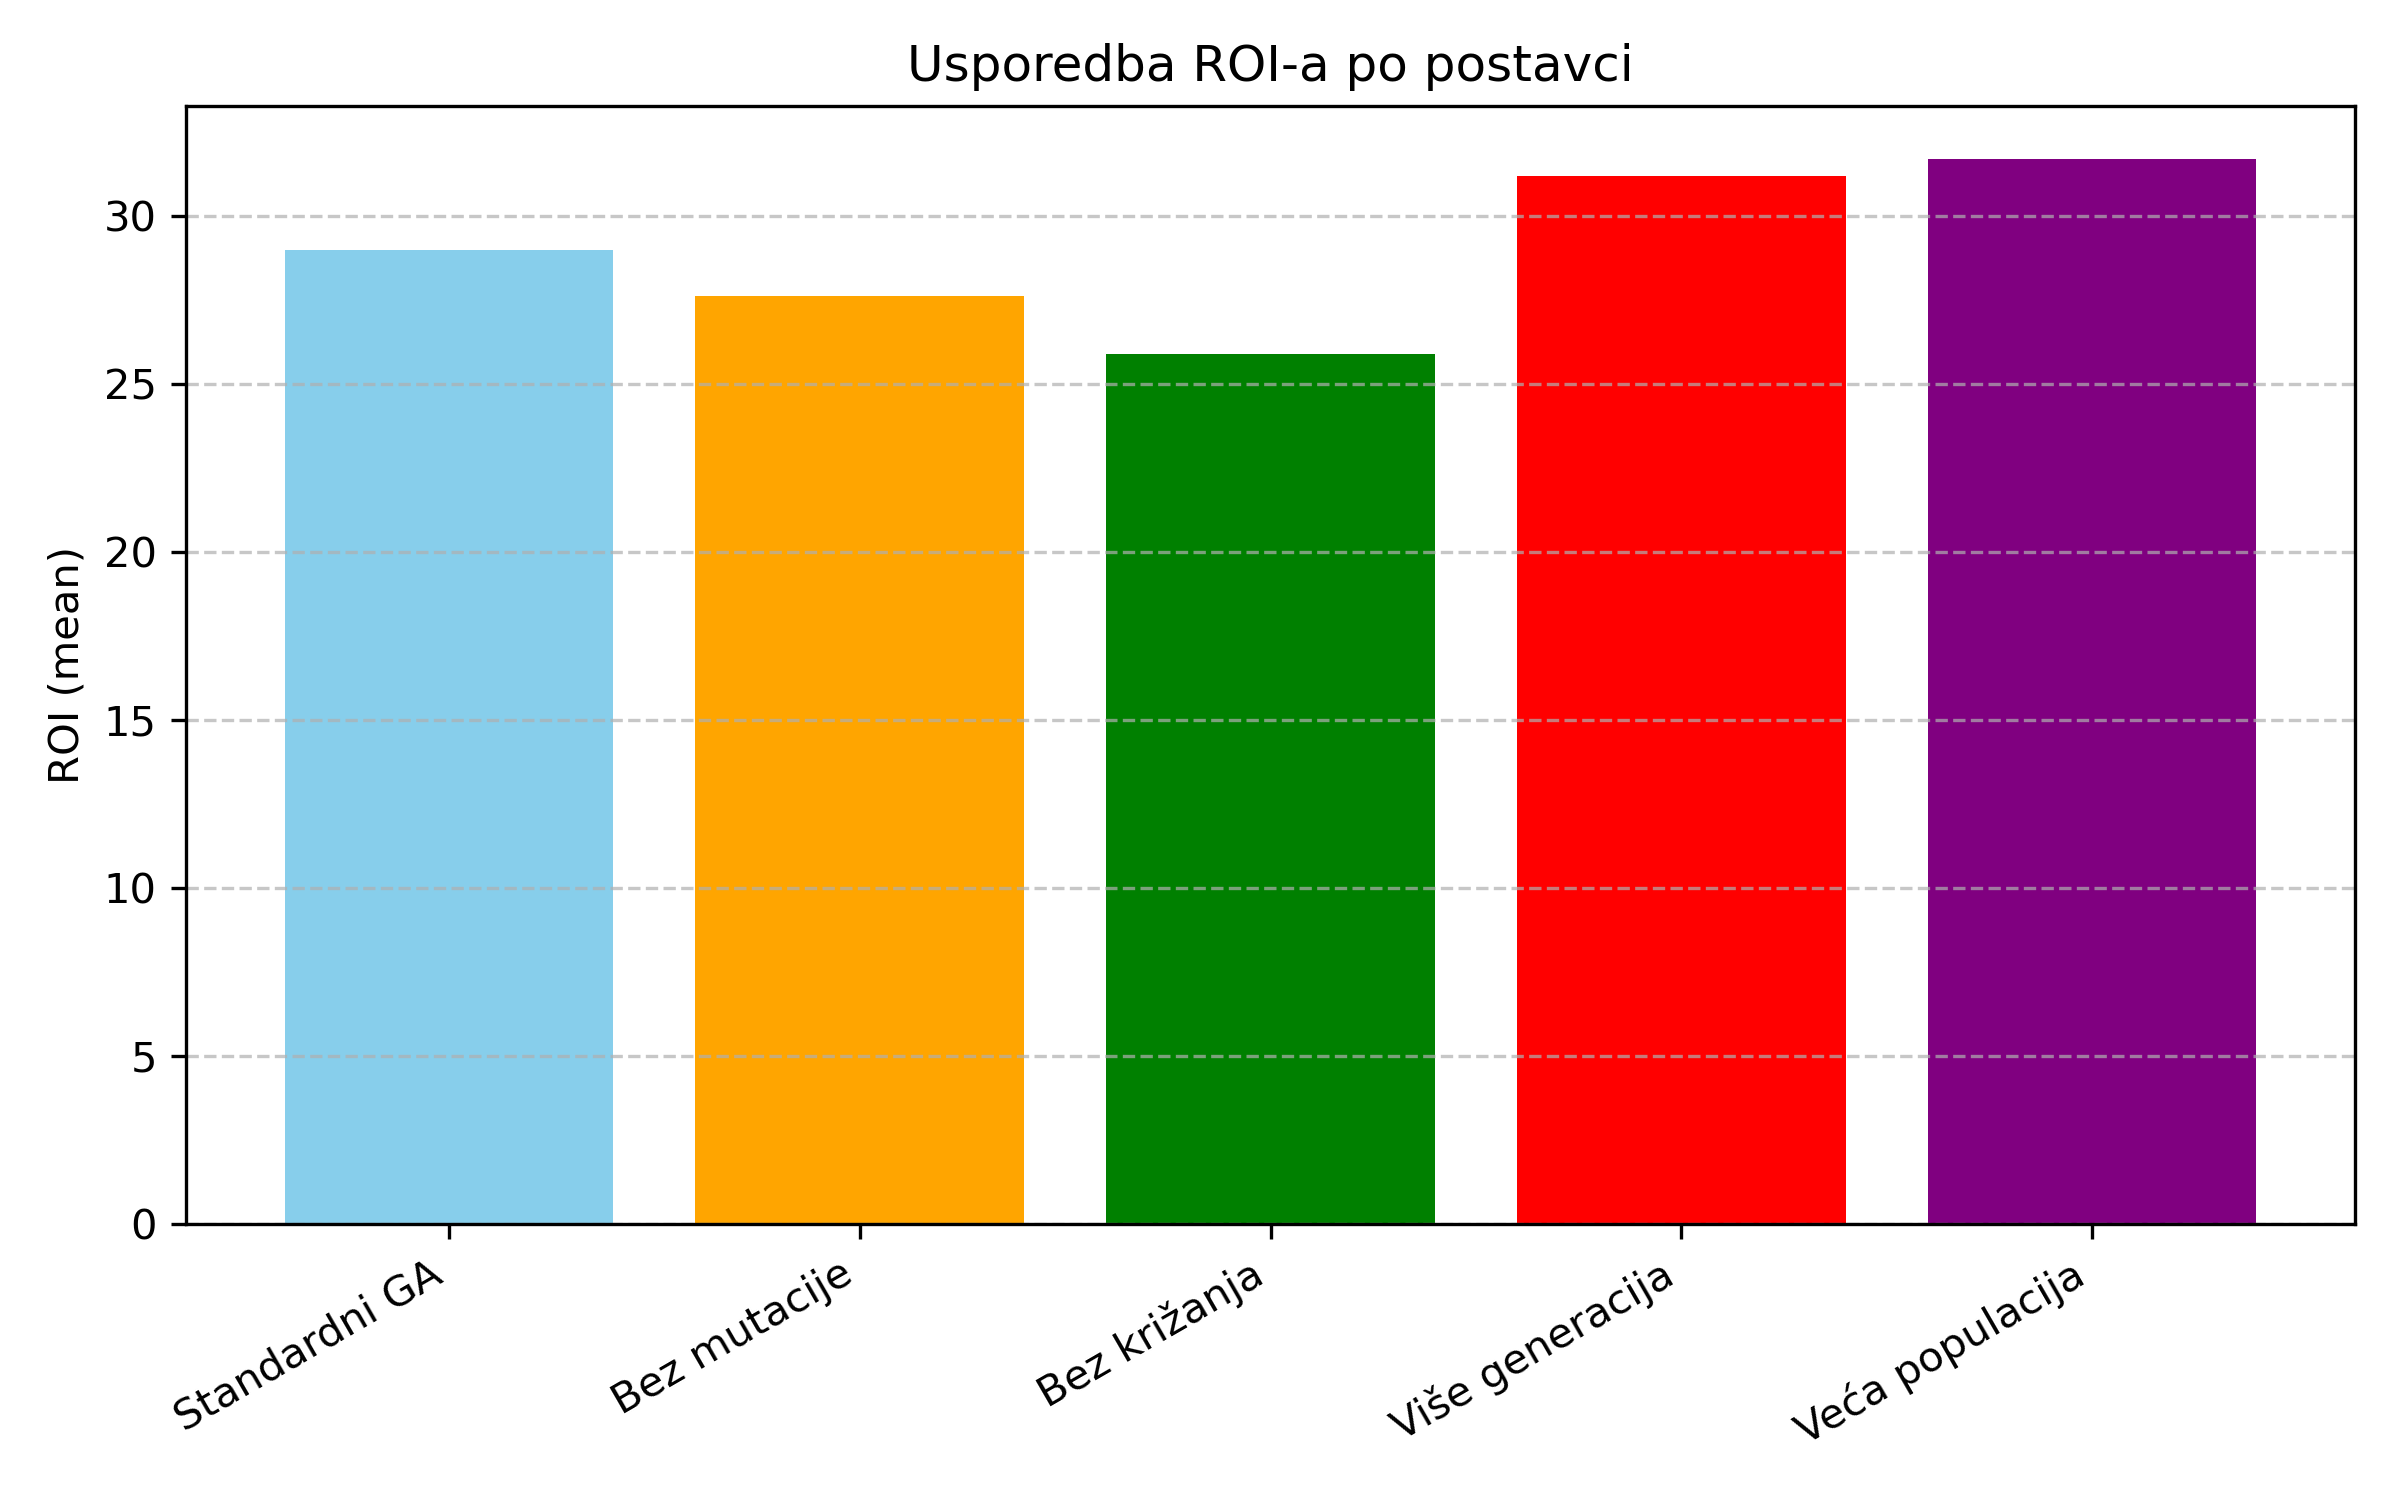
\includegraphics[width=\textwidth]{slike/ga_usporedba_roi.png}
        \caption{Usporedba prosječnog ROI-a.}
        \label{fig:ga_roi}
    \end{subfigure}
    \hfill
    \begin{subfigure}[b]{0.48\textwidth}
        \centering
        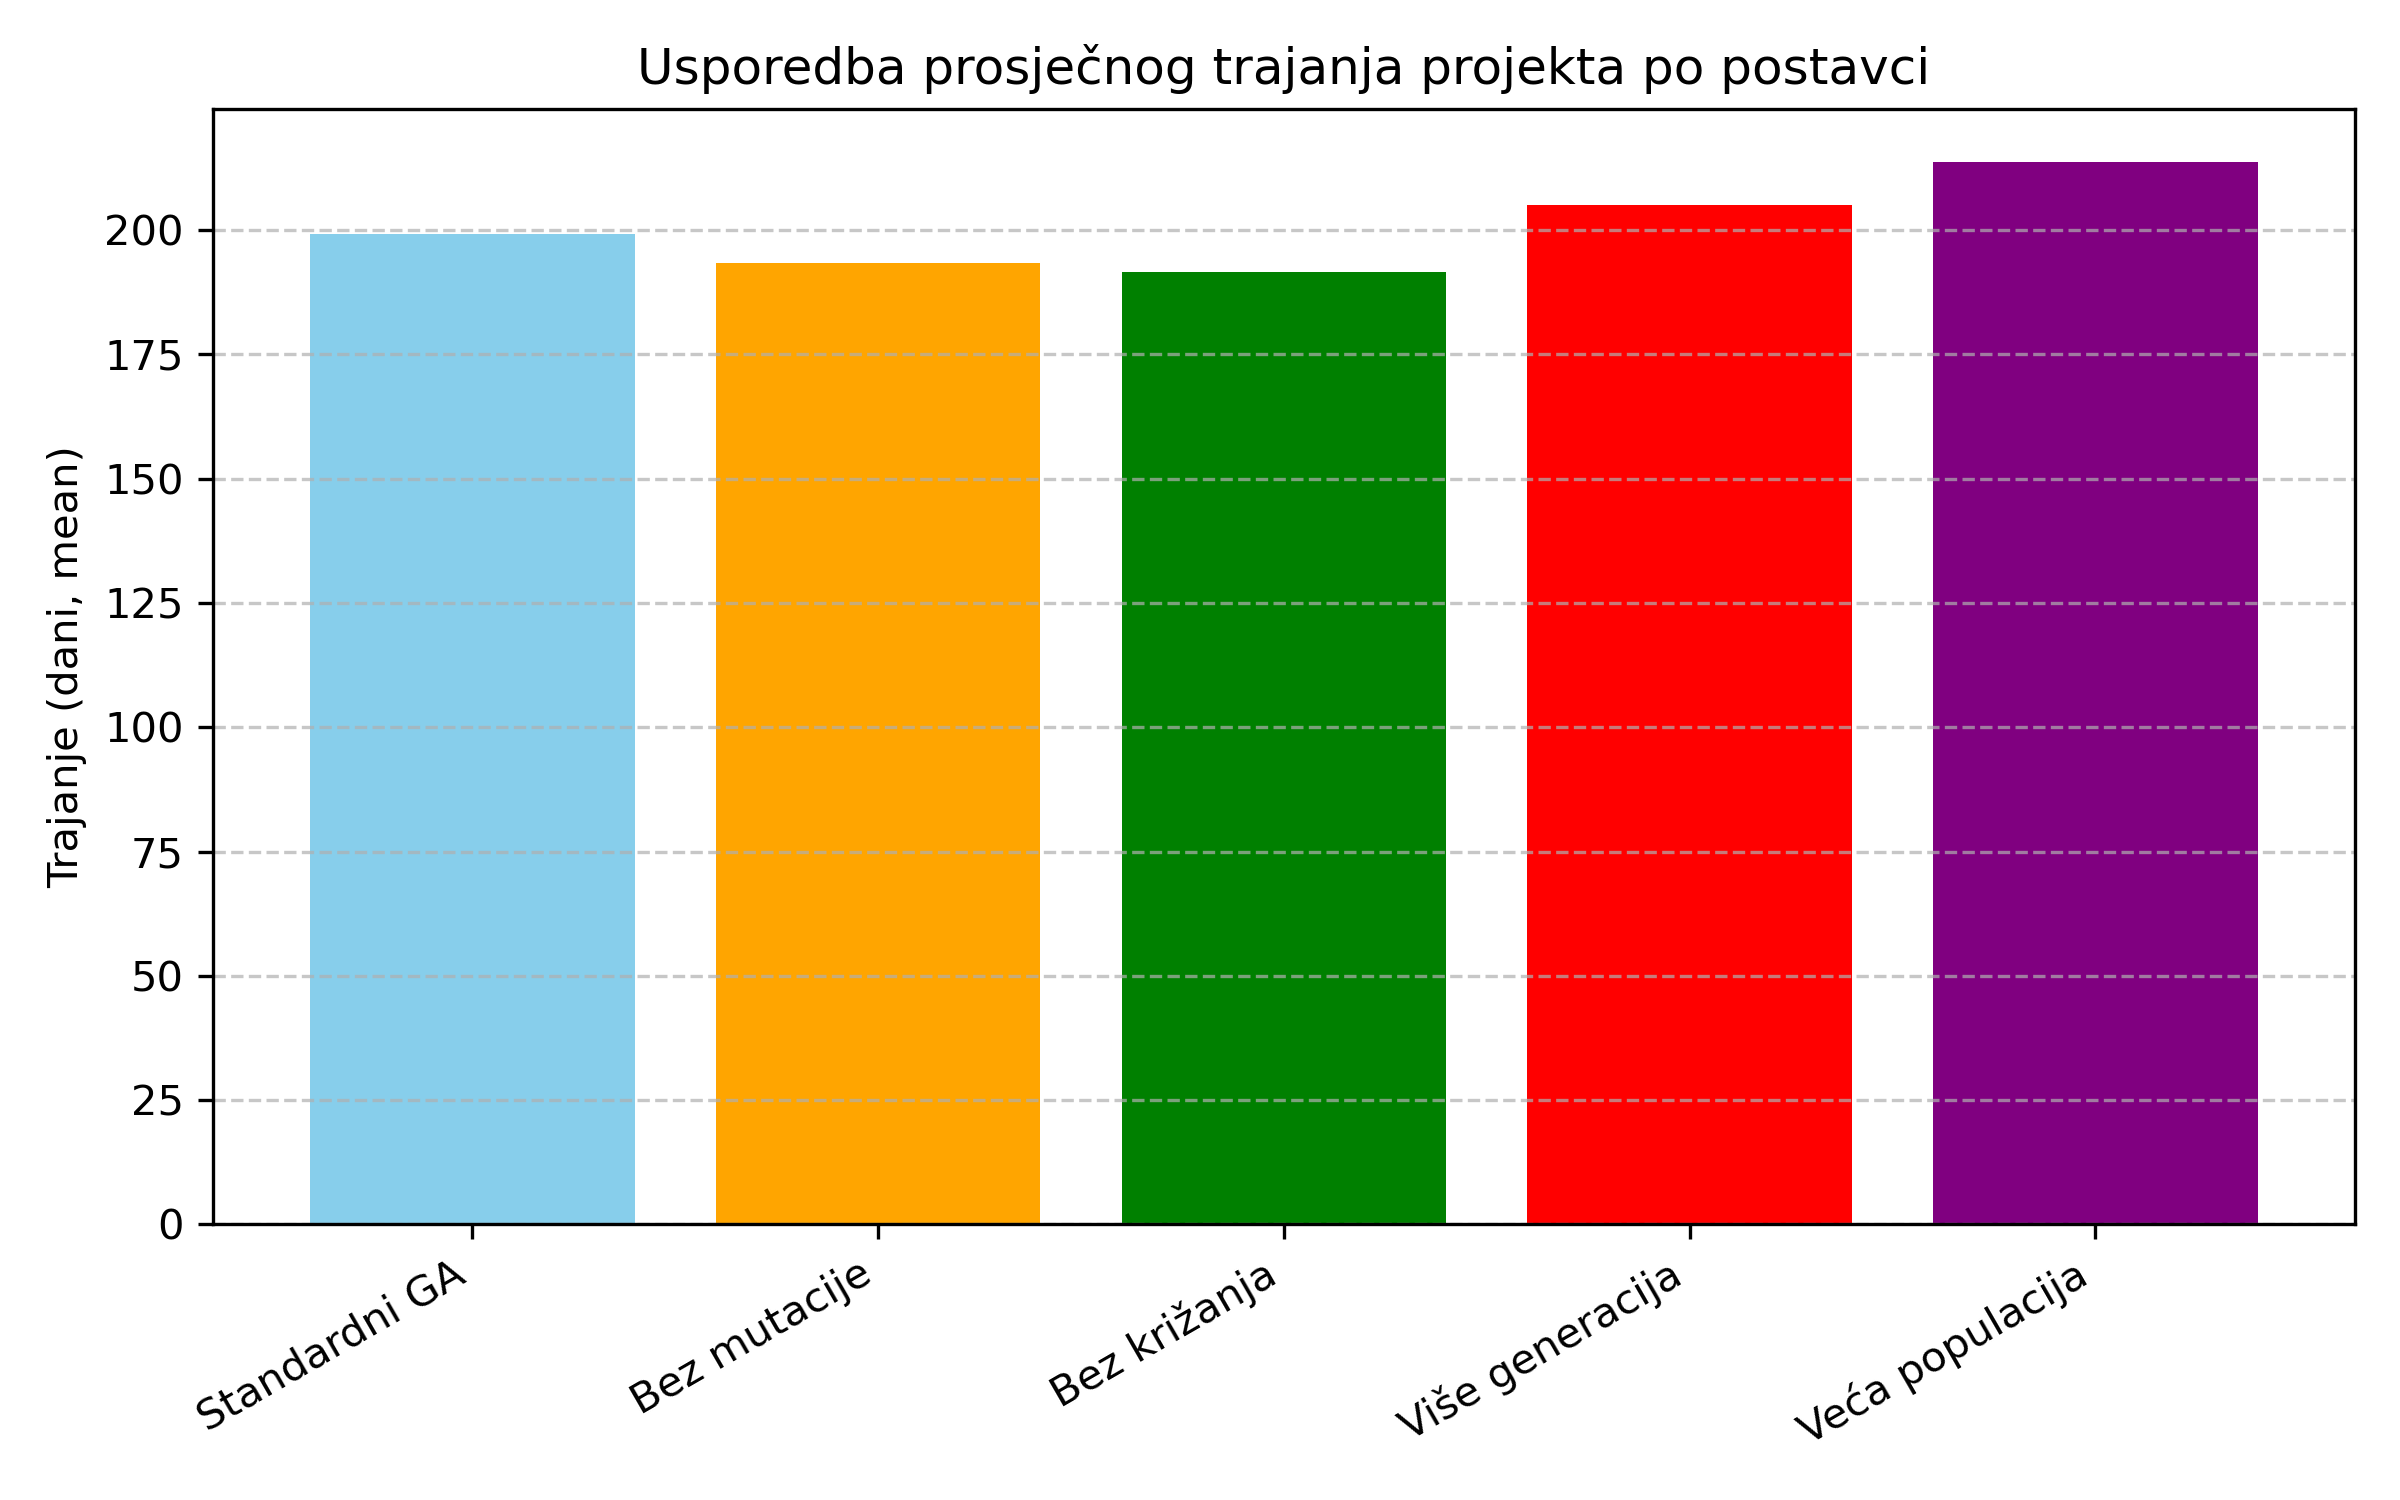
\includegraphics[width=\textwidth]{slike/ga_usporedba_trajanje.png}
        \caption{Usporedba prosječnog trajanja.}
        \label{fig:ga_trajanje}
    \end{subfigure}
    \caption{Grafički prikaz rezultata ablacijske studije za genetski algoritam.}
    \label{fig:ga_ablation}
\end{figure}

\textbf{Zaključak Eksperimenta 1:}
Na temelju empirijskih rezultata, konfiguracija \emph{Veća populacija} odabrana je kao ``šampionska''. Njezini parametri (\texttt{POP\_SIZE = 200}, \texttt{NGEN = 40}, itd.) poslužili su kao osnova za definiranje parametara u drugoj fazi istraživanja, uz nužne prilagodbe resursa s obzirom na složenost problema.

\subsection{Eksperiment 2: Usporedna analiza optimizacijskih modela}
Druga faza istraživanja čini ključnu eksperimentalnu provjeru glavne hipoteze rada. Koristeći kalibrirane parametre iz Eksperimenta 1, provedena je sustavna usporedba triju razvijenih modela prema planu definiranom u Tablici~\ref{tab:plan_eksperimenata}.

\begin{table}[H]
    \centering
    \caption{Plan naprednih eksperimenata.}
    \label{tab:plan_eksperimenata}
    \resizebox{\textwidth}{!}{
    \begin{tabular}{|l|l|l|l|l|}
        \hline
        \textbf{Eksperiment} & \textbf{NUM\_ACTIVITIES} & \textbf{BUDGET} & \textbf{Pripada seriji} & \textbf{Napomena} \\
        \hline
        A1 & 10 & 1000 & A & Osnovna složenost \\
        \hline
        A2 / B2 & 50 & 2500 & A, B & Centralni / Referentni eksperiment \\
        \hline
        A3 & 100 & 5000 & A & Visoka složenost \\
        \hline
        B1 & 50 & 1500 & B & Restriktivan budžet \\
        \hline
        B3 & 50 & 4000 & B & Labav budžet \\
        \hline
    \end{tabular}
    }
\end{table}

\subsubsection{Rezultati}
Svi rezultati dobiveni provođenjem Eksperimenta 2 sažeti su u Tablici~\ref{tab:rezultati}. Ova tablica predstavlja temelj za daljnju diskusiju.

\begin{table}[H]
    \centering
    \caption{Konačni rezultati usporedne analize optimizacijskih modela.}
    \label{tab:rezultati}
    \resizebox{\textwidth}{!}{
    \begin{tabular}{|l|l|c|c|c|c|}
        \hline
        \textbf{Eksperiment} & \textbf{Scenarij} & \textbf{ROI\_mean} & \textbf{ROI\_std} & \textbf{Trajanje\_mean} & \textbf{Trajanje\_std} \\
        \hline
        A1\_Osnovni & Random Search (MC) & 17.140 & 3.55e-15 & 144.151 & 0.911 \\
        A1\_Osnovni & GA (samo ROI) & 17.140 & 3.55e-15 & 143.103 & 1.239 \\
        A1\_Osnovni & GA+MC (NSGA-II) & 17.140 & 3.55e-15 & 142.003 & 0.372 \\
        \hline
        A2\_Srednji & Random Search (MC) & 40.108 & 0.703 & 341.024 & 9.405 \\
        A2\_Srednji & GA (samo ROI) & 46.125 & 0.412 & 363.632 & 7.843 \\
        A2\_Srednji & GA+MC (NSGA-II) & 44.099 & 0.980 & 319.210 & 13.171 \\
        \hline
        A3\_Slozeni & Random Search (MC) & 95.835 & 1.468 & 715.604 & 10.451 \\
        A3\_Slozeni & GA (samo ROI) & 114.224 & 0.891 & 792.300 & 11.933 \\
        A3\_Slozeni & GA+MC (NSGA-II) & 109.095 & 2.008 & 681.565 & 21.733 \\
        \hline
        B1\_Restriktivan & Random Search (MC) & 24.120 & 1.846 & 197.621 & 20.181 \\
        B1\_Restriktivan & GA (samo ROI) & 37.976 & 0.567 & 253.562 & 12.386 \\
        B1\_Restriktivan & GA+MC (NSGA-II) & 17.711 & 17.728 & 50104.382 & 49894.619 \\
        \hline
        B3\_Labav & Random Search (MC) & 71.379 & 1.114 & 536.901 & 16.247 \\
        B3\_Labav & GA (samo ROI) & 79.065 & 0.518 & 562.191 & 9.345 \\
        B3\_Labav & GA+MC (NSGA-II) & 76.949 & 0.487 & 526.612 & 10.602 \\
        \hline
    \end{tabular}
    }
\end{table}

\subsubsection{Diskusija rezultata}
Dobiveni rezultati analizirani su kroz tematske cjeline, s ciljem odgovaranja na postavljena istraživačka pitanja.

\textbf{Analiza Skalabilnosti (Serija A)}
Kao što je vidljivo na Slici~\ref{fig:a_skalabilnost}, porast složenosti problema drastično utječe na performanse modela. Jaz u \textbf{ROI\_mean} vrijednostima eksponencijalno raste u korist genetskih algoritama, potvrđujući hipotezu o nužnosti inteligentne pretrage (H1). Ovakav nalaz, gdje metaheuristički pristupi značajno nadmašuju nasumičnu pretragu na složenim problemima, u skladu je s rezultatima koje su dobili i drugi istraživači u srodnim domenama primjene \cite{Gandomi2013}. Istovremeno, analiza trajanja otkriva postojanje kompromisa: hibridni model GA+MC (NSGA-II) konzistentno identificira rješenja sa značajno nižim prosječnim trajanjem, potvrđujući hipotezu H2.

\begin{figure}[H]
    \centering
    \begin{subfigure}[b]{0.48\textwidth}
        \centering
        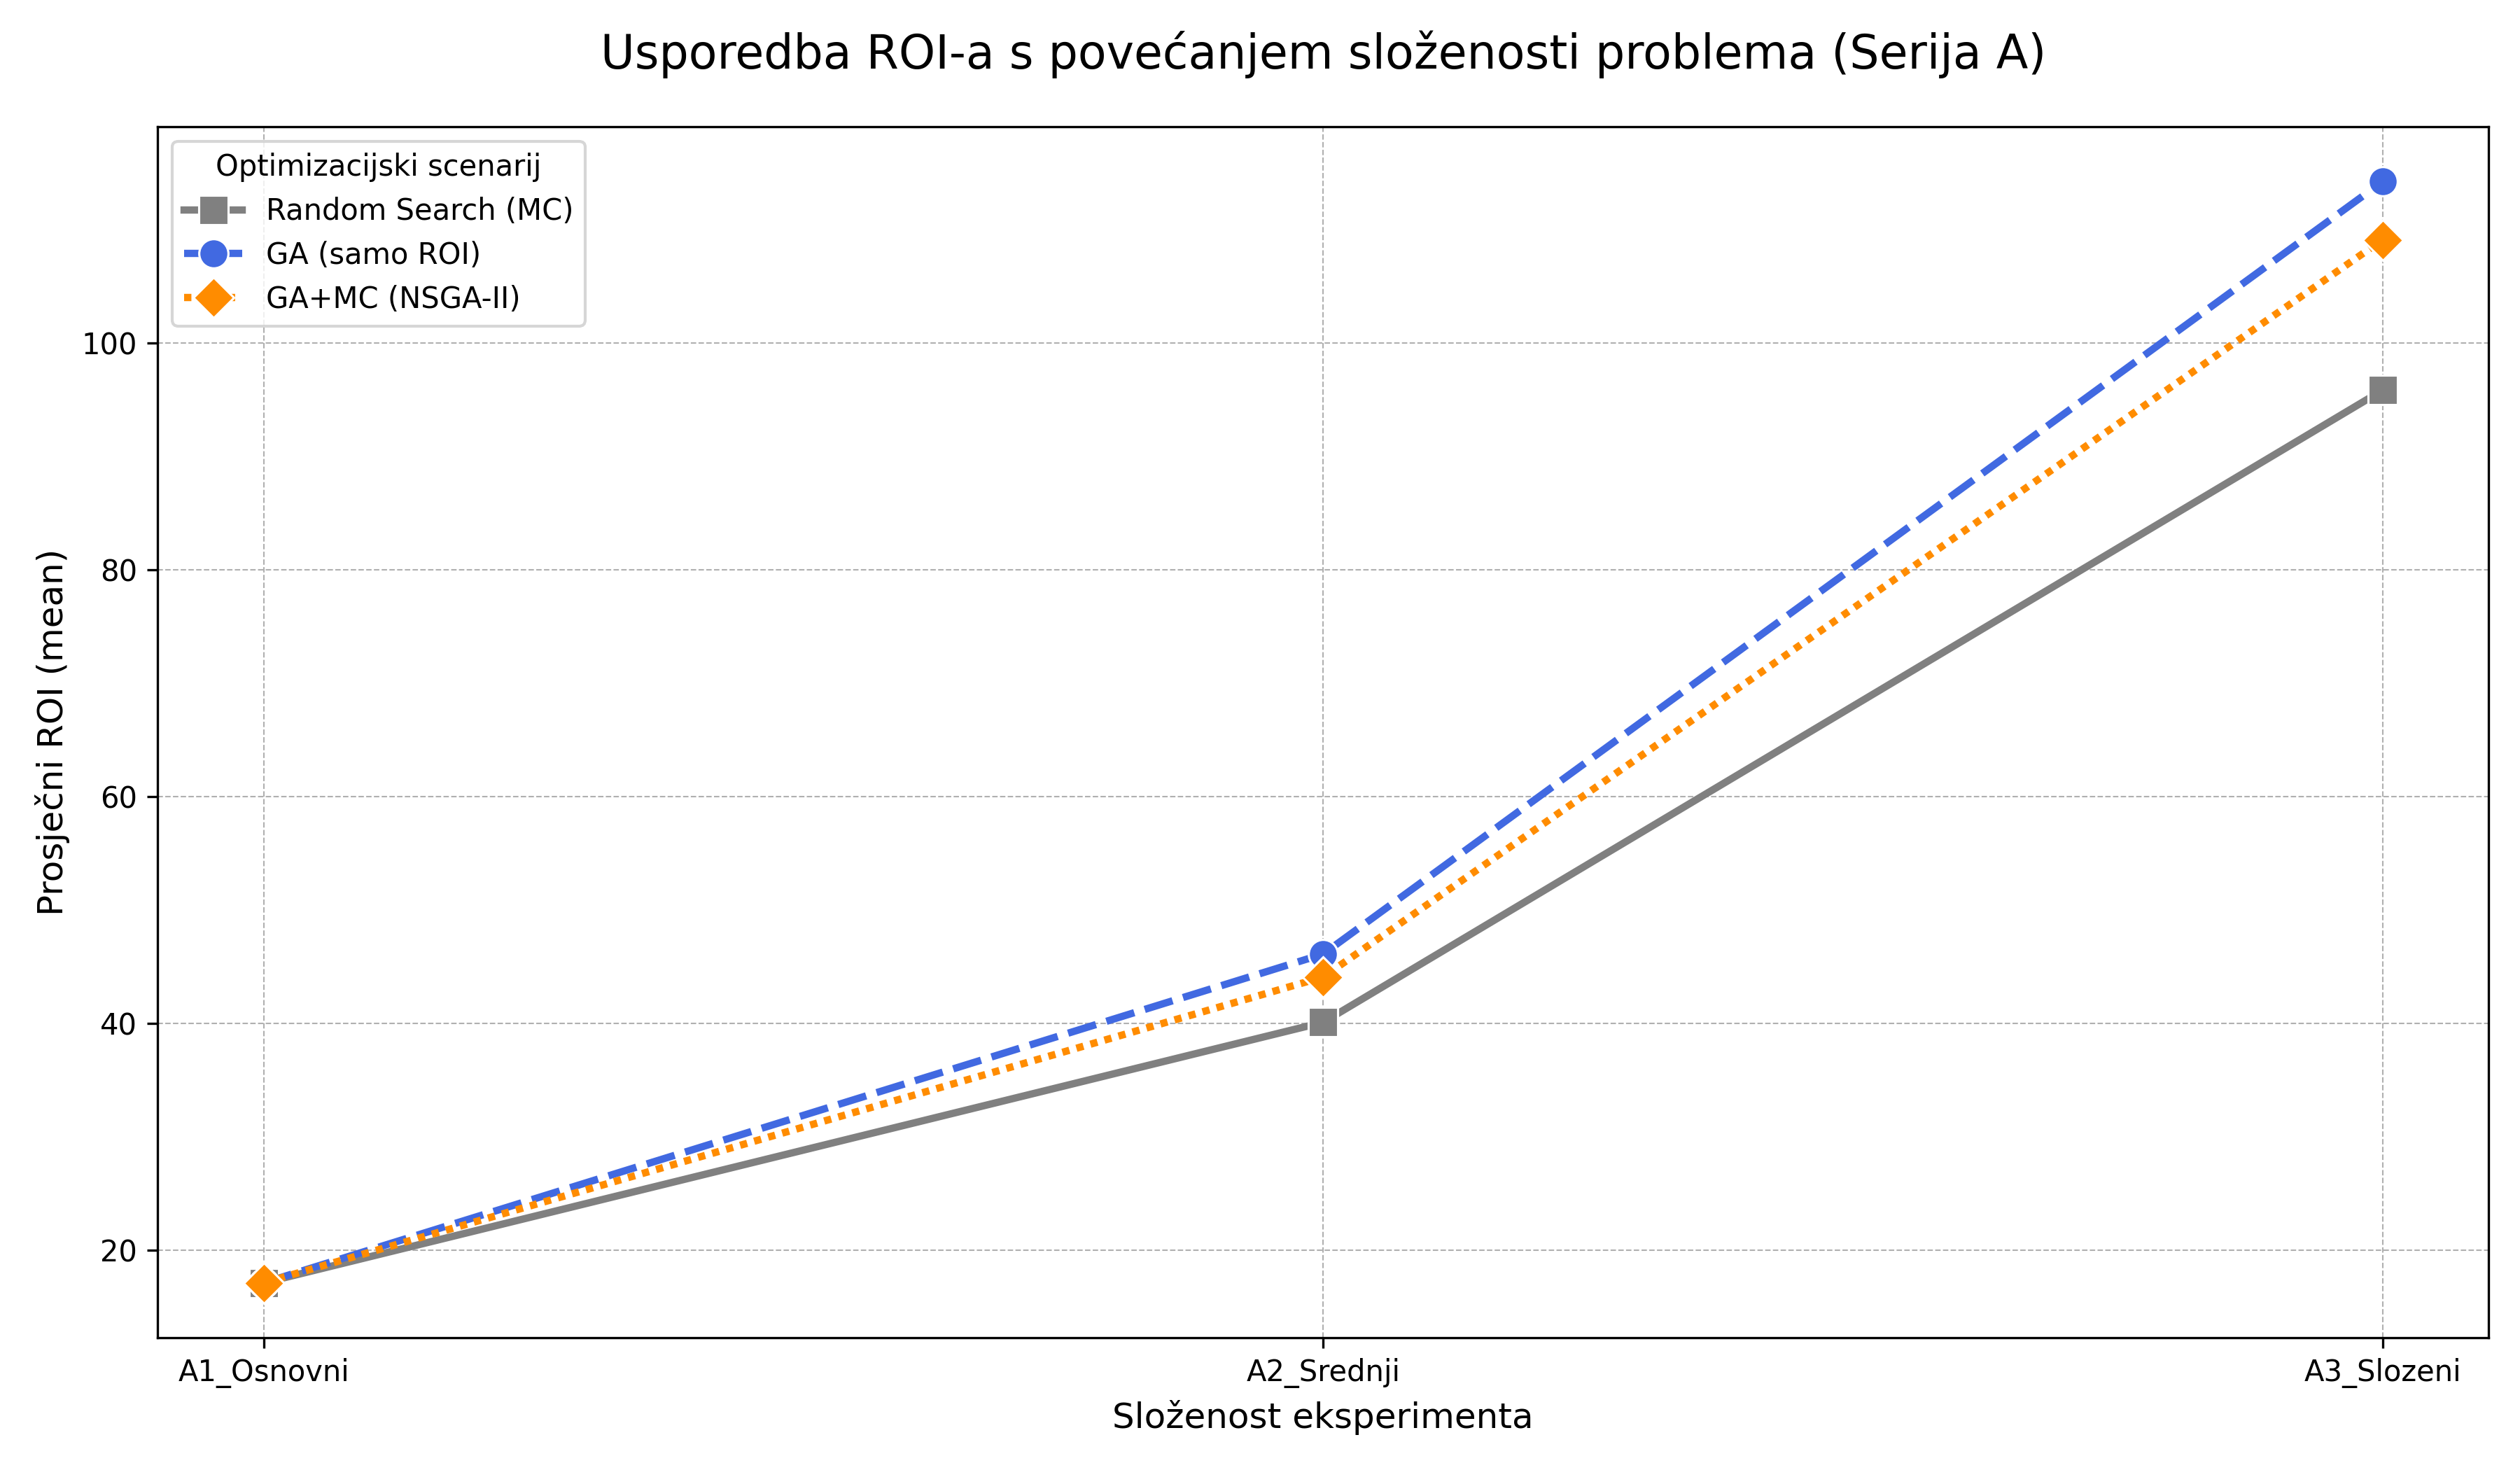
\includegraphics[width=\textwidth]{slike/grafikoni_final/A_skalabilnost_roi.png}
        \caption{Usporedba prosječnog ROI-a.}
    \end{subfigure}
    \hfill
    \begin{subfigure}[b]{0.48\textwidth}
        \centering
        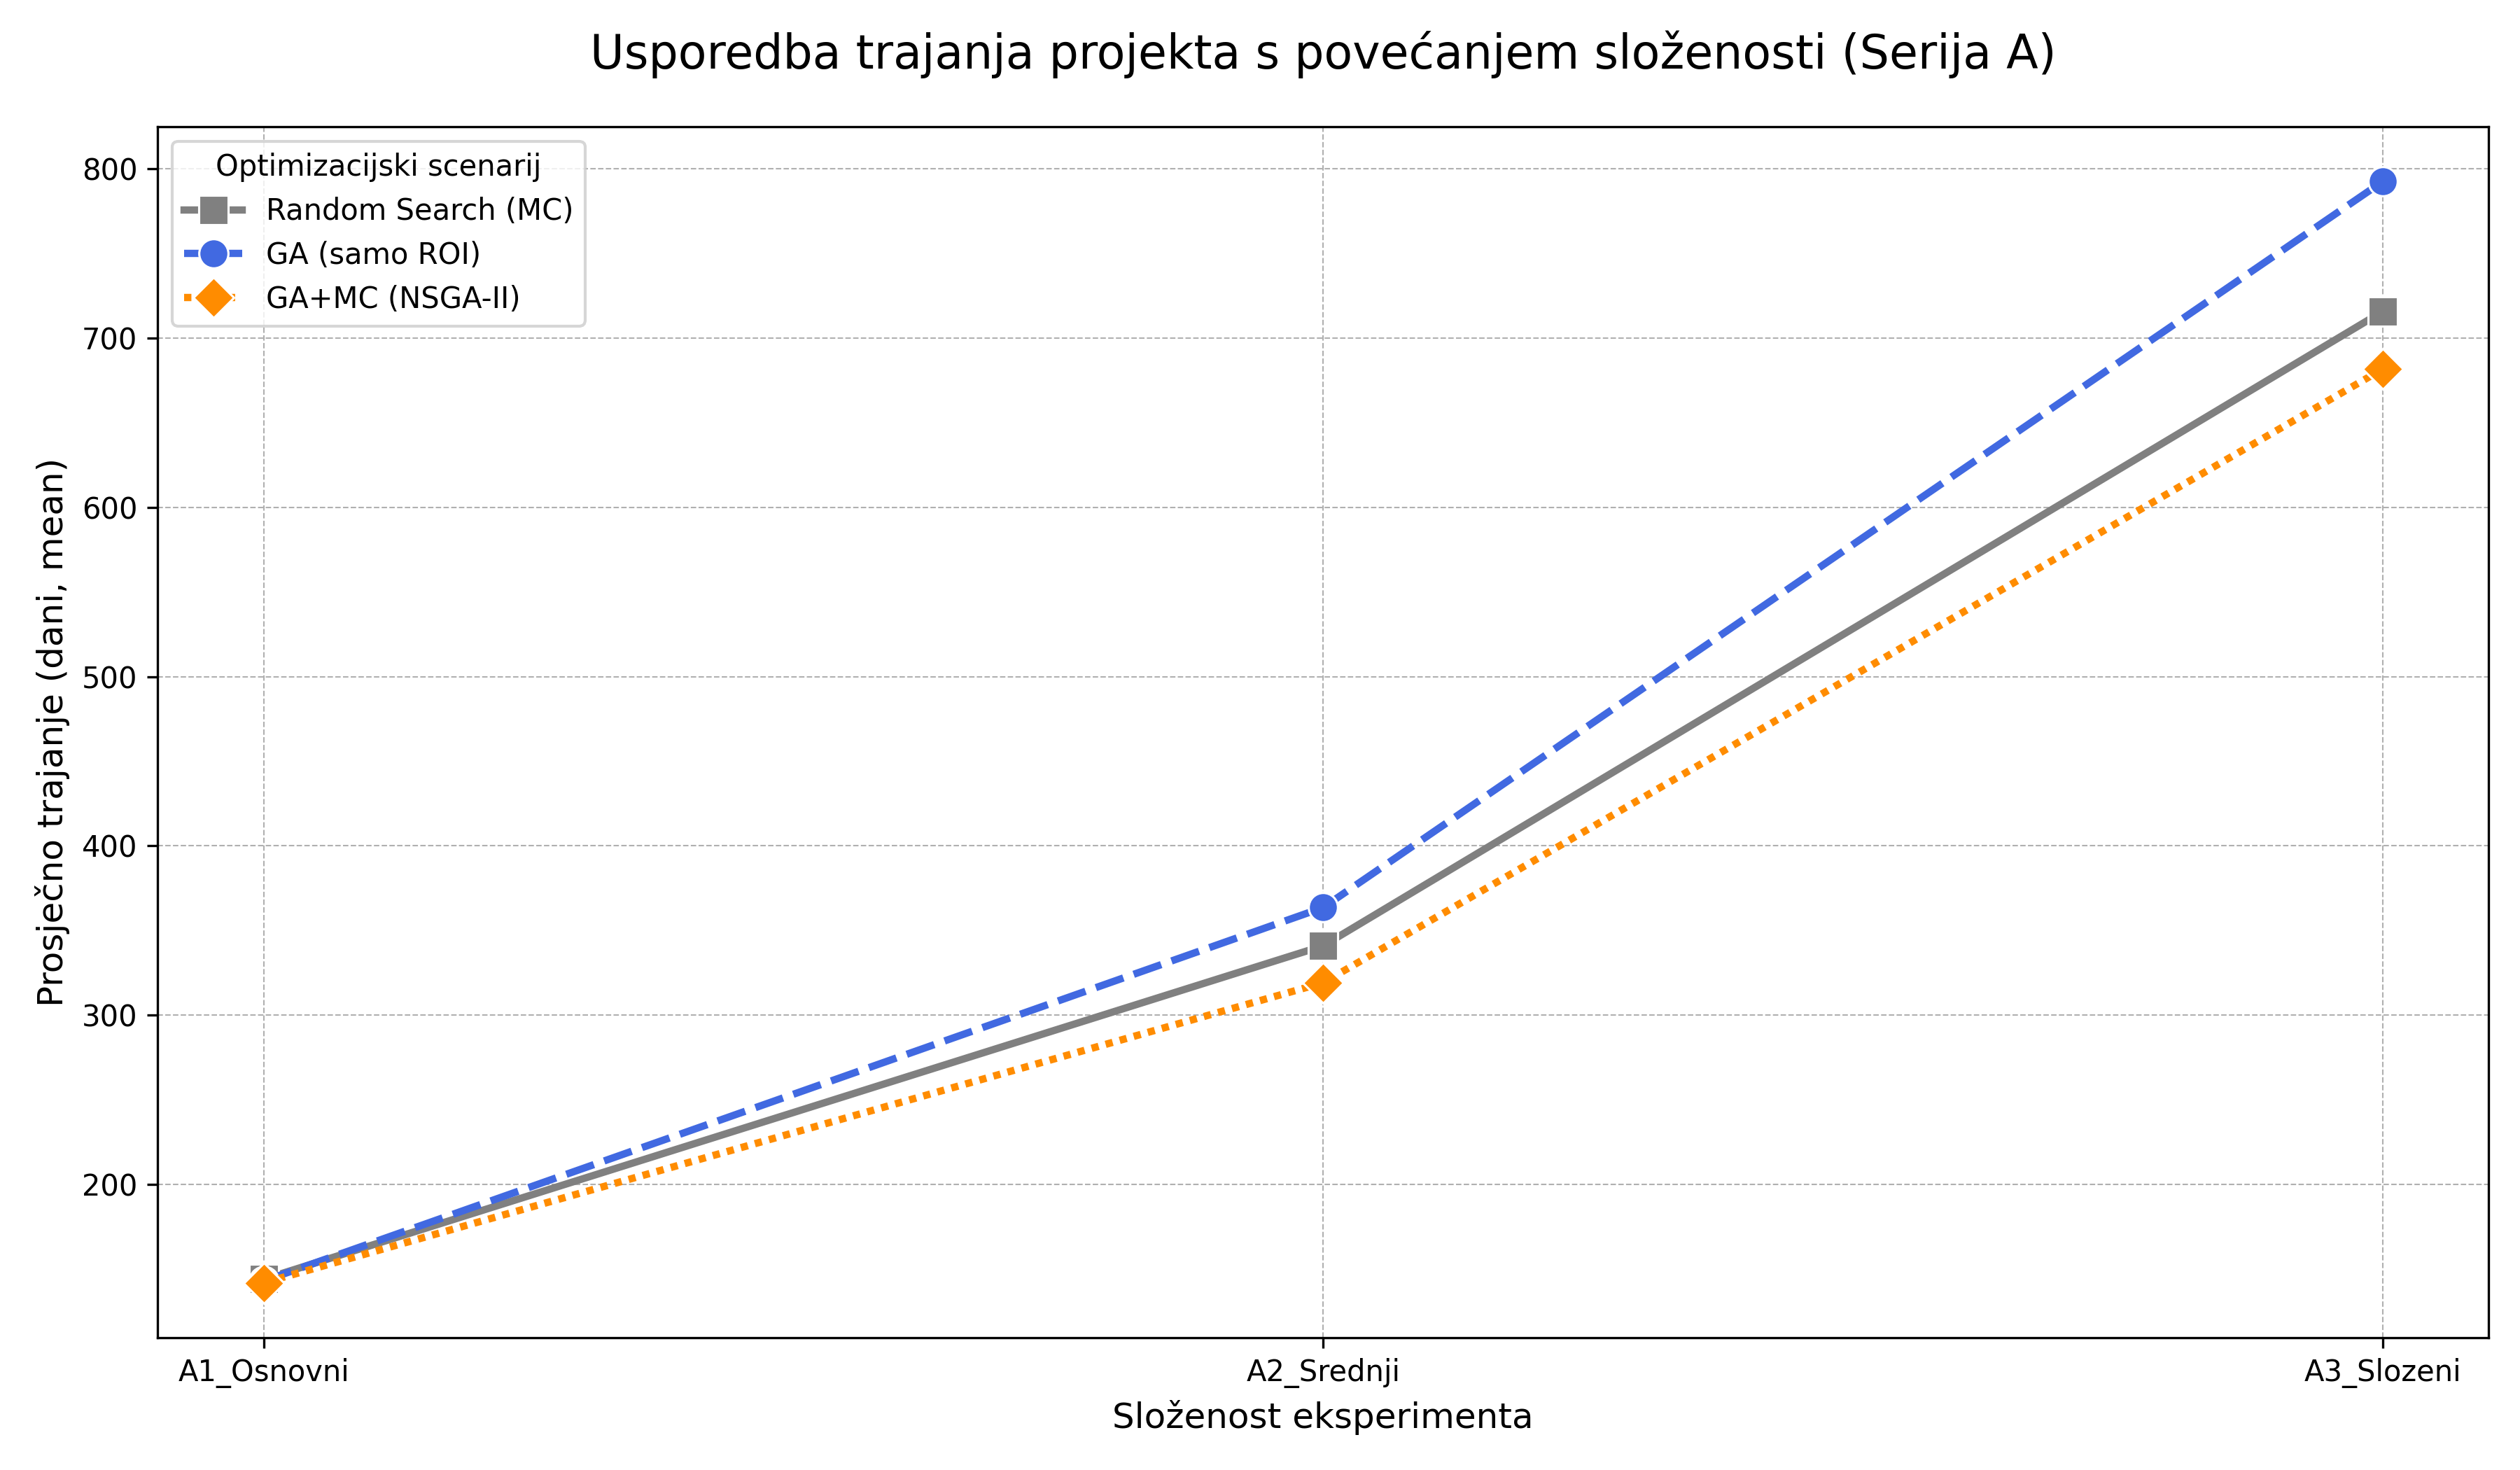
\includegraphics[width=\textwidth]{slike/grafikoni_final/A_skalabilnost_trajanje.png}
        \caption{Usporedba prosječnog trajanja.}
    \end{subfigure}
    \caption{Grafički prikaz rezultata Serije A: Usporedba modela u uvjetima rastuće složenosti.}
    \label{fig:a_skalabilnost}
\end{figure}

\textbf{Analiza Utjecaja Ograničenja (Serija B)}
Slika~\ref{fig:budzet_roi} ilustrira ponašanje modela pod različitim proračunskim pritiskom. Najvažniji nalaz dolazi iz eksperimenta s restriktivnim budžetom (B1), gdje GA+MC (NSGA-II) pokazuje iznimnu krhkost, ne uspijevajući pronaći valjano rješenje u 50\% pokretanja. S druge strane, jednostavniji GA (samo ROI) pokazuje se vrlo robusnim. Ovo ukazuje da složenost više-kriterijske pretrage može biti nedostatak u ekstremno suženim prostorima rješenja. U uvjetima labavog budžeta (B3), svi modeli rade očekivano dobro, potvrđujući hipotezu H3.

\begin{figure}[H]
    \centering
    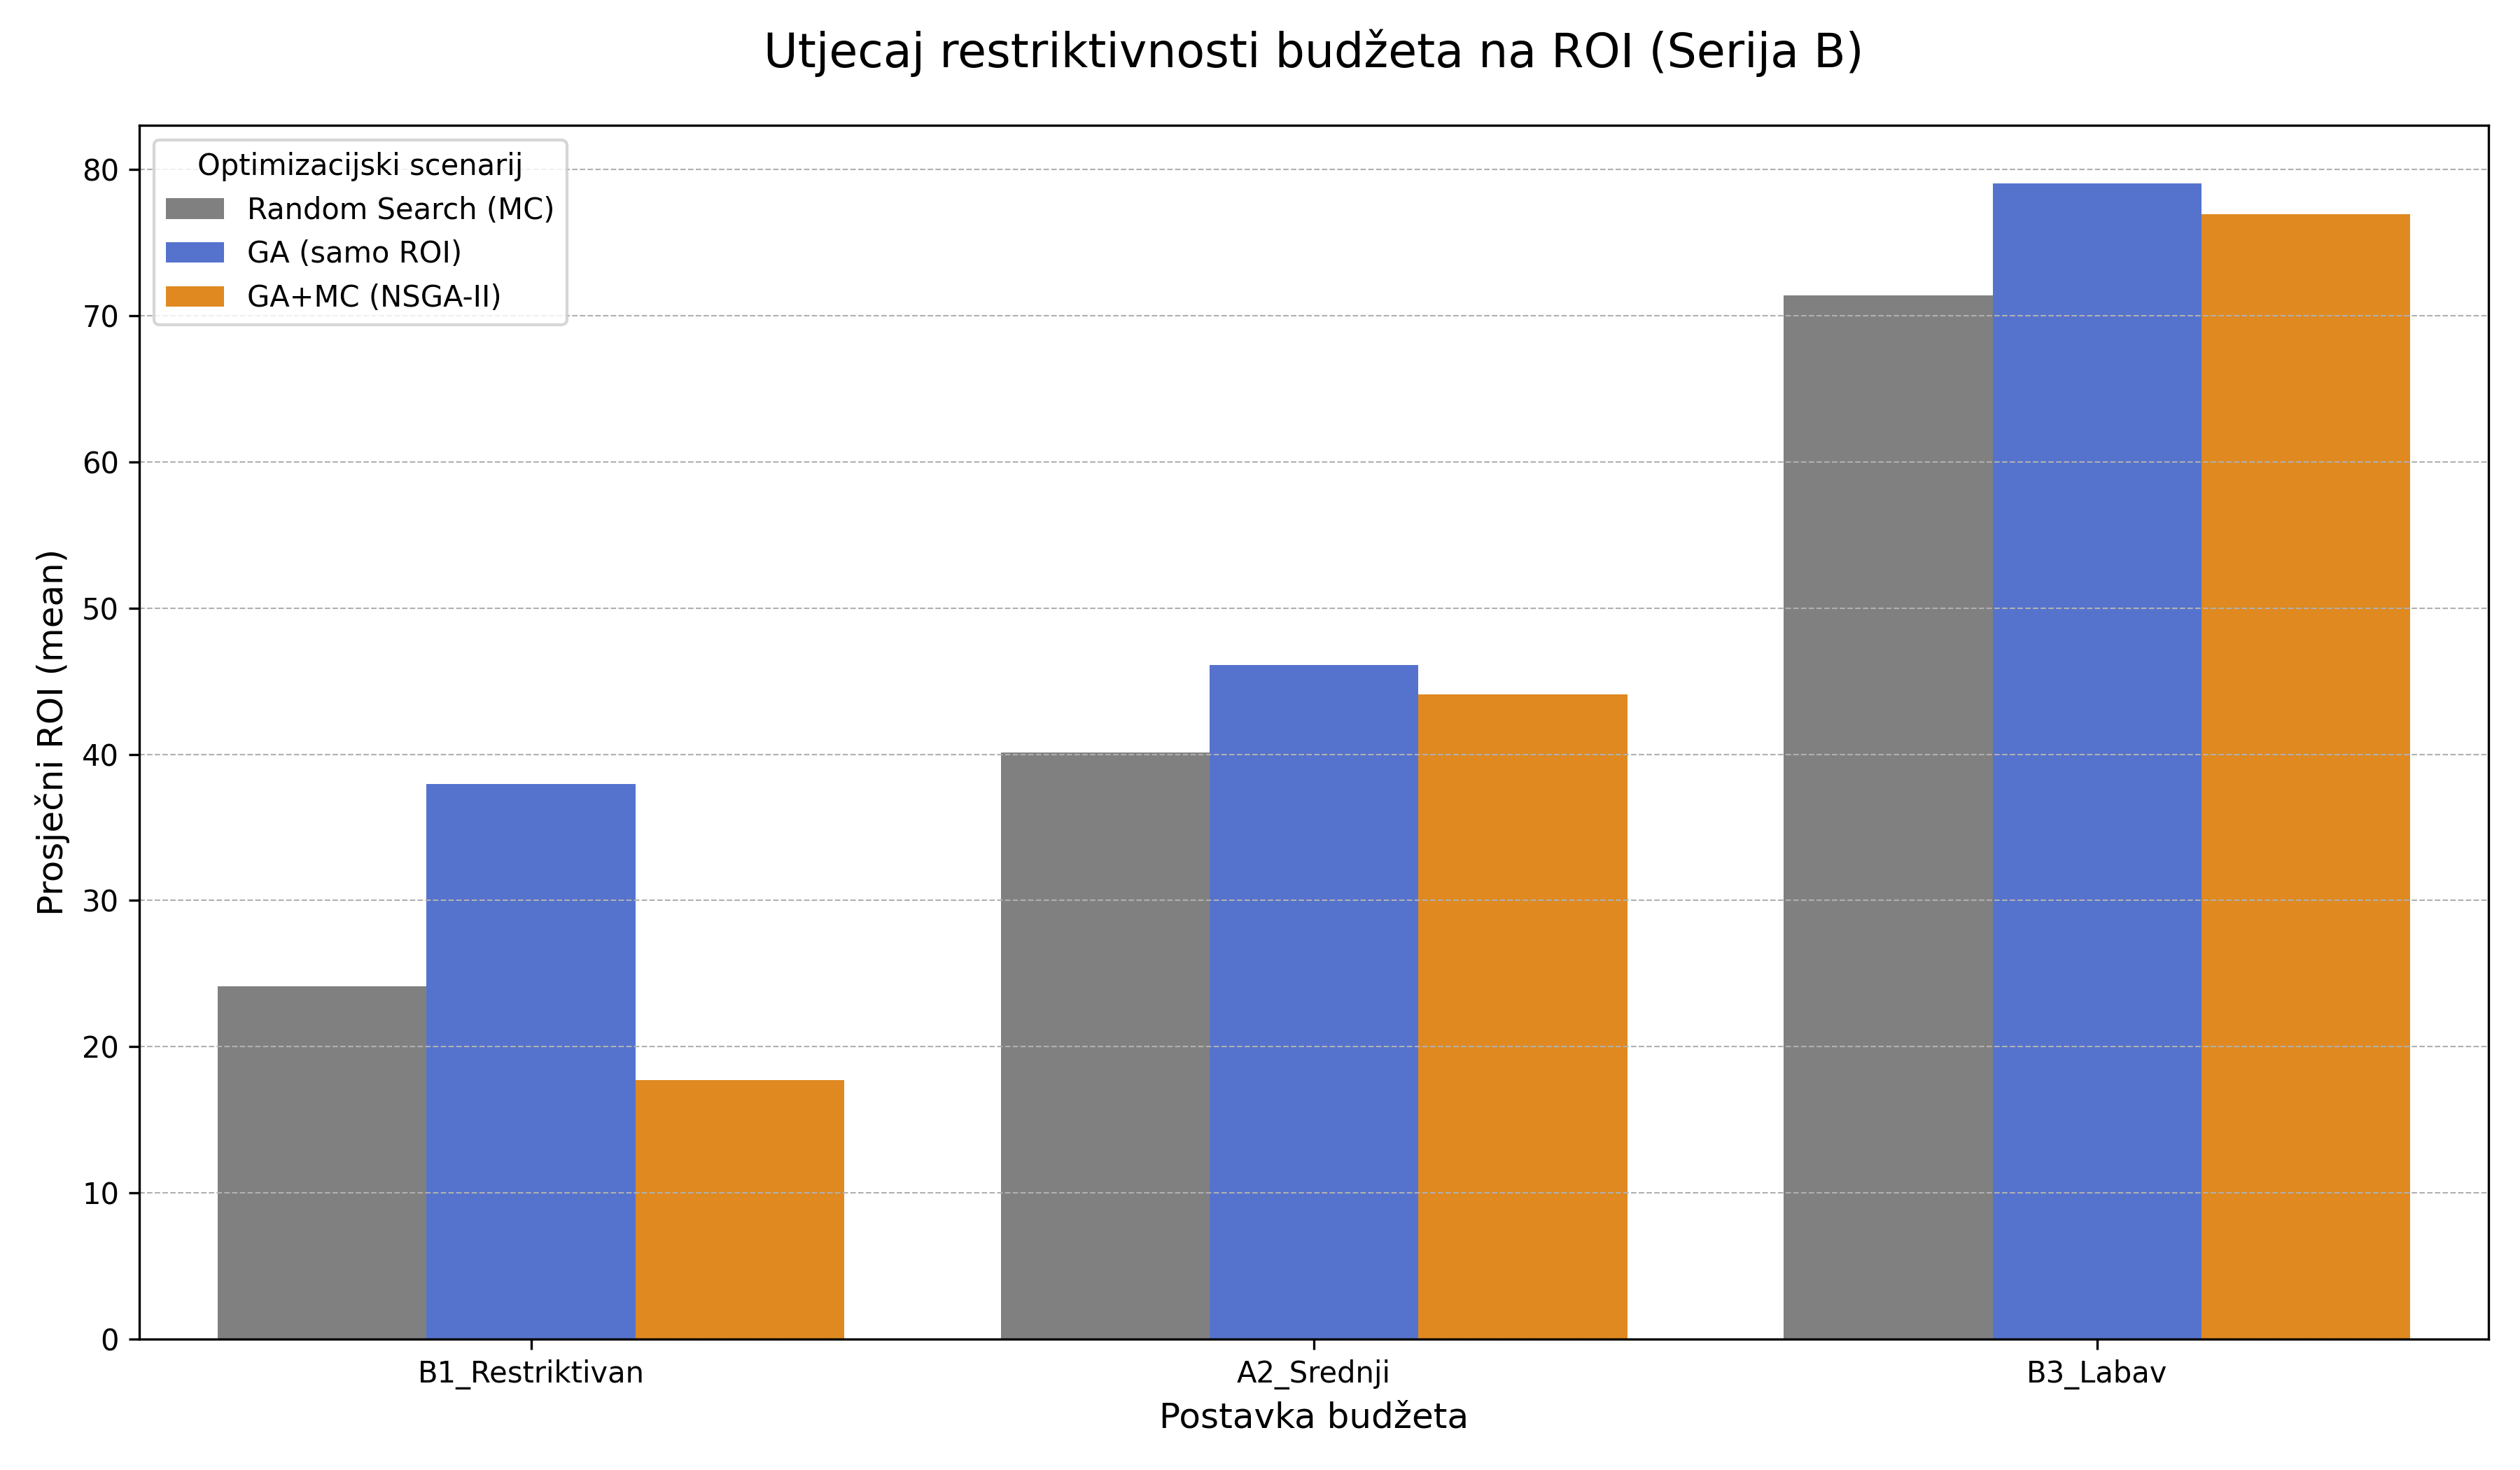
\includegraphics[width=0.8\textwidth]{slike/grafikoni_final/B_budzet_roi.png}
    \caption{Usporedba prosječnog ROI-a modela pod različitim proračunskim ograničenjima (Serija B).}
    \label{fig:budzet_roi}
\end{figure}

\textbf{Analiza Stabilnosti i Pouzdanosti}
Grafikoni na Slici~\ref{fig:stabilnost} prikazuju standardnu devijaciju kao mjeru konzistentnosti. Izvan scenarija B1 gdje je doživio neuspjeh, GA+MC (NSGA-II) model pokazuje usporedivu ili nižu devijaciju trajanja u odnosu na klasični GA. To implicira da rješenja koja nudi nisu samo u prosjeku brža, već su i pouzdanija.

\begin{figure}[H]
    \centering
    \begin{subfigure}[b]{0.48\textwidth}
        \centering
        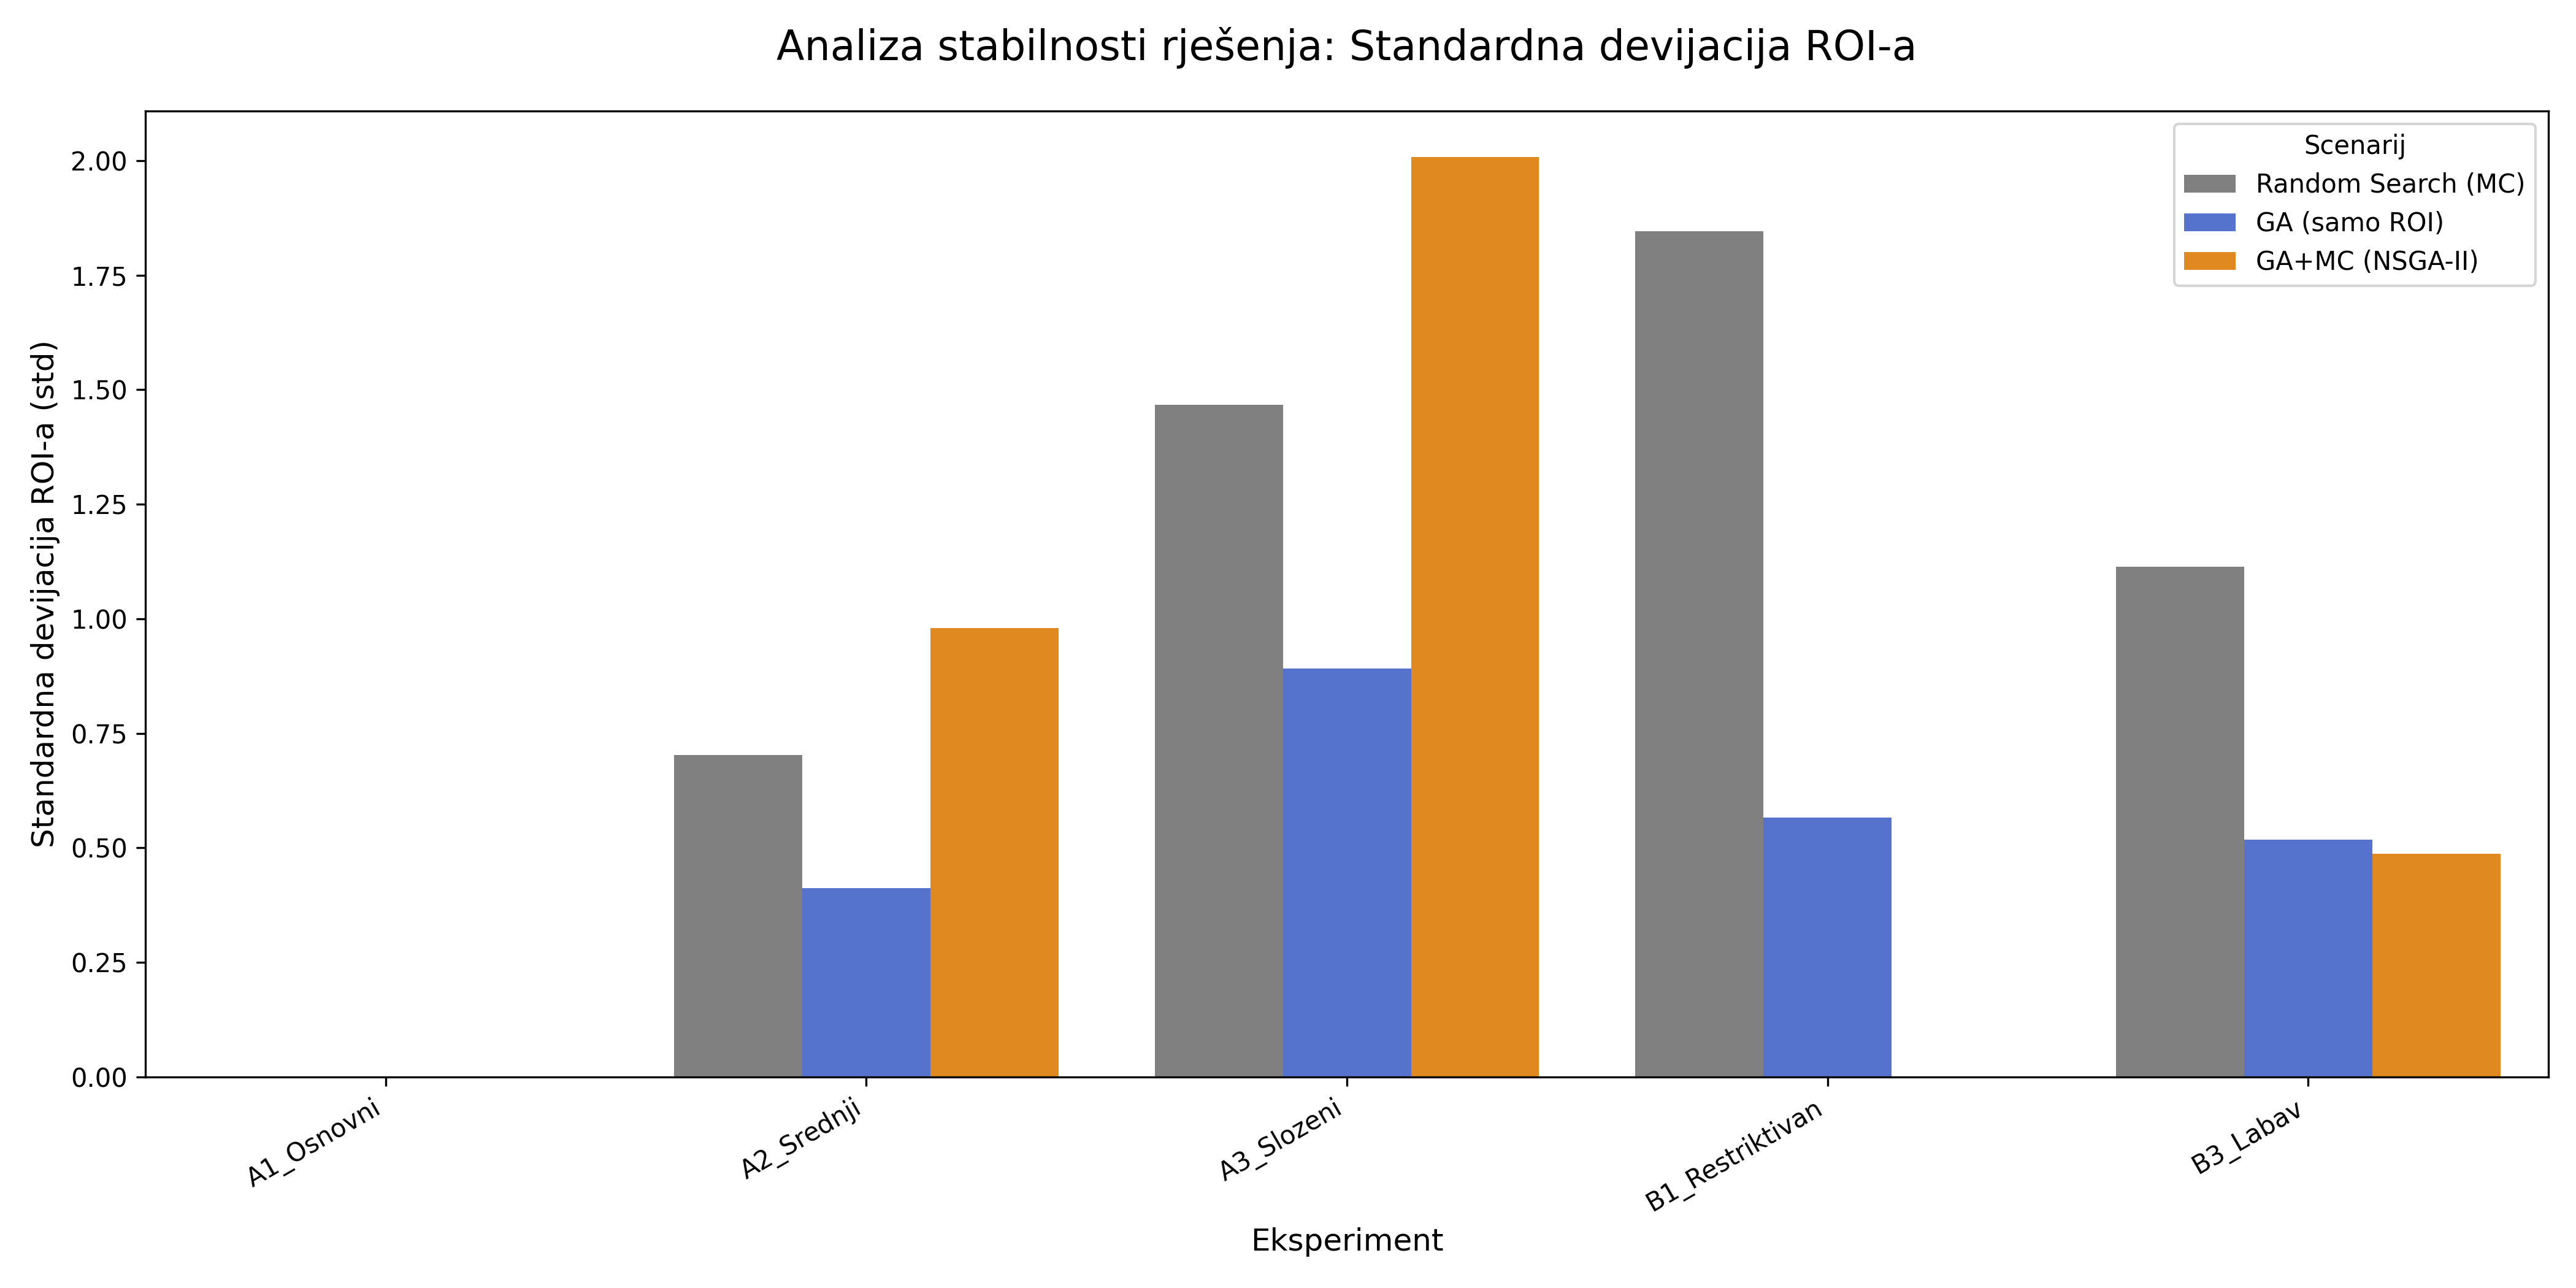
\includegraphics[width=\textwidth]{slike/grafikoni_final/C_stabilnost_roi.png}
        \caption{Stabilnost ROI-a.}
    \end{subfigure}
    \hfill
    \begin{subfigure}[b]{0.48\textwidth}
        \centering
        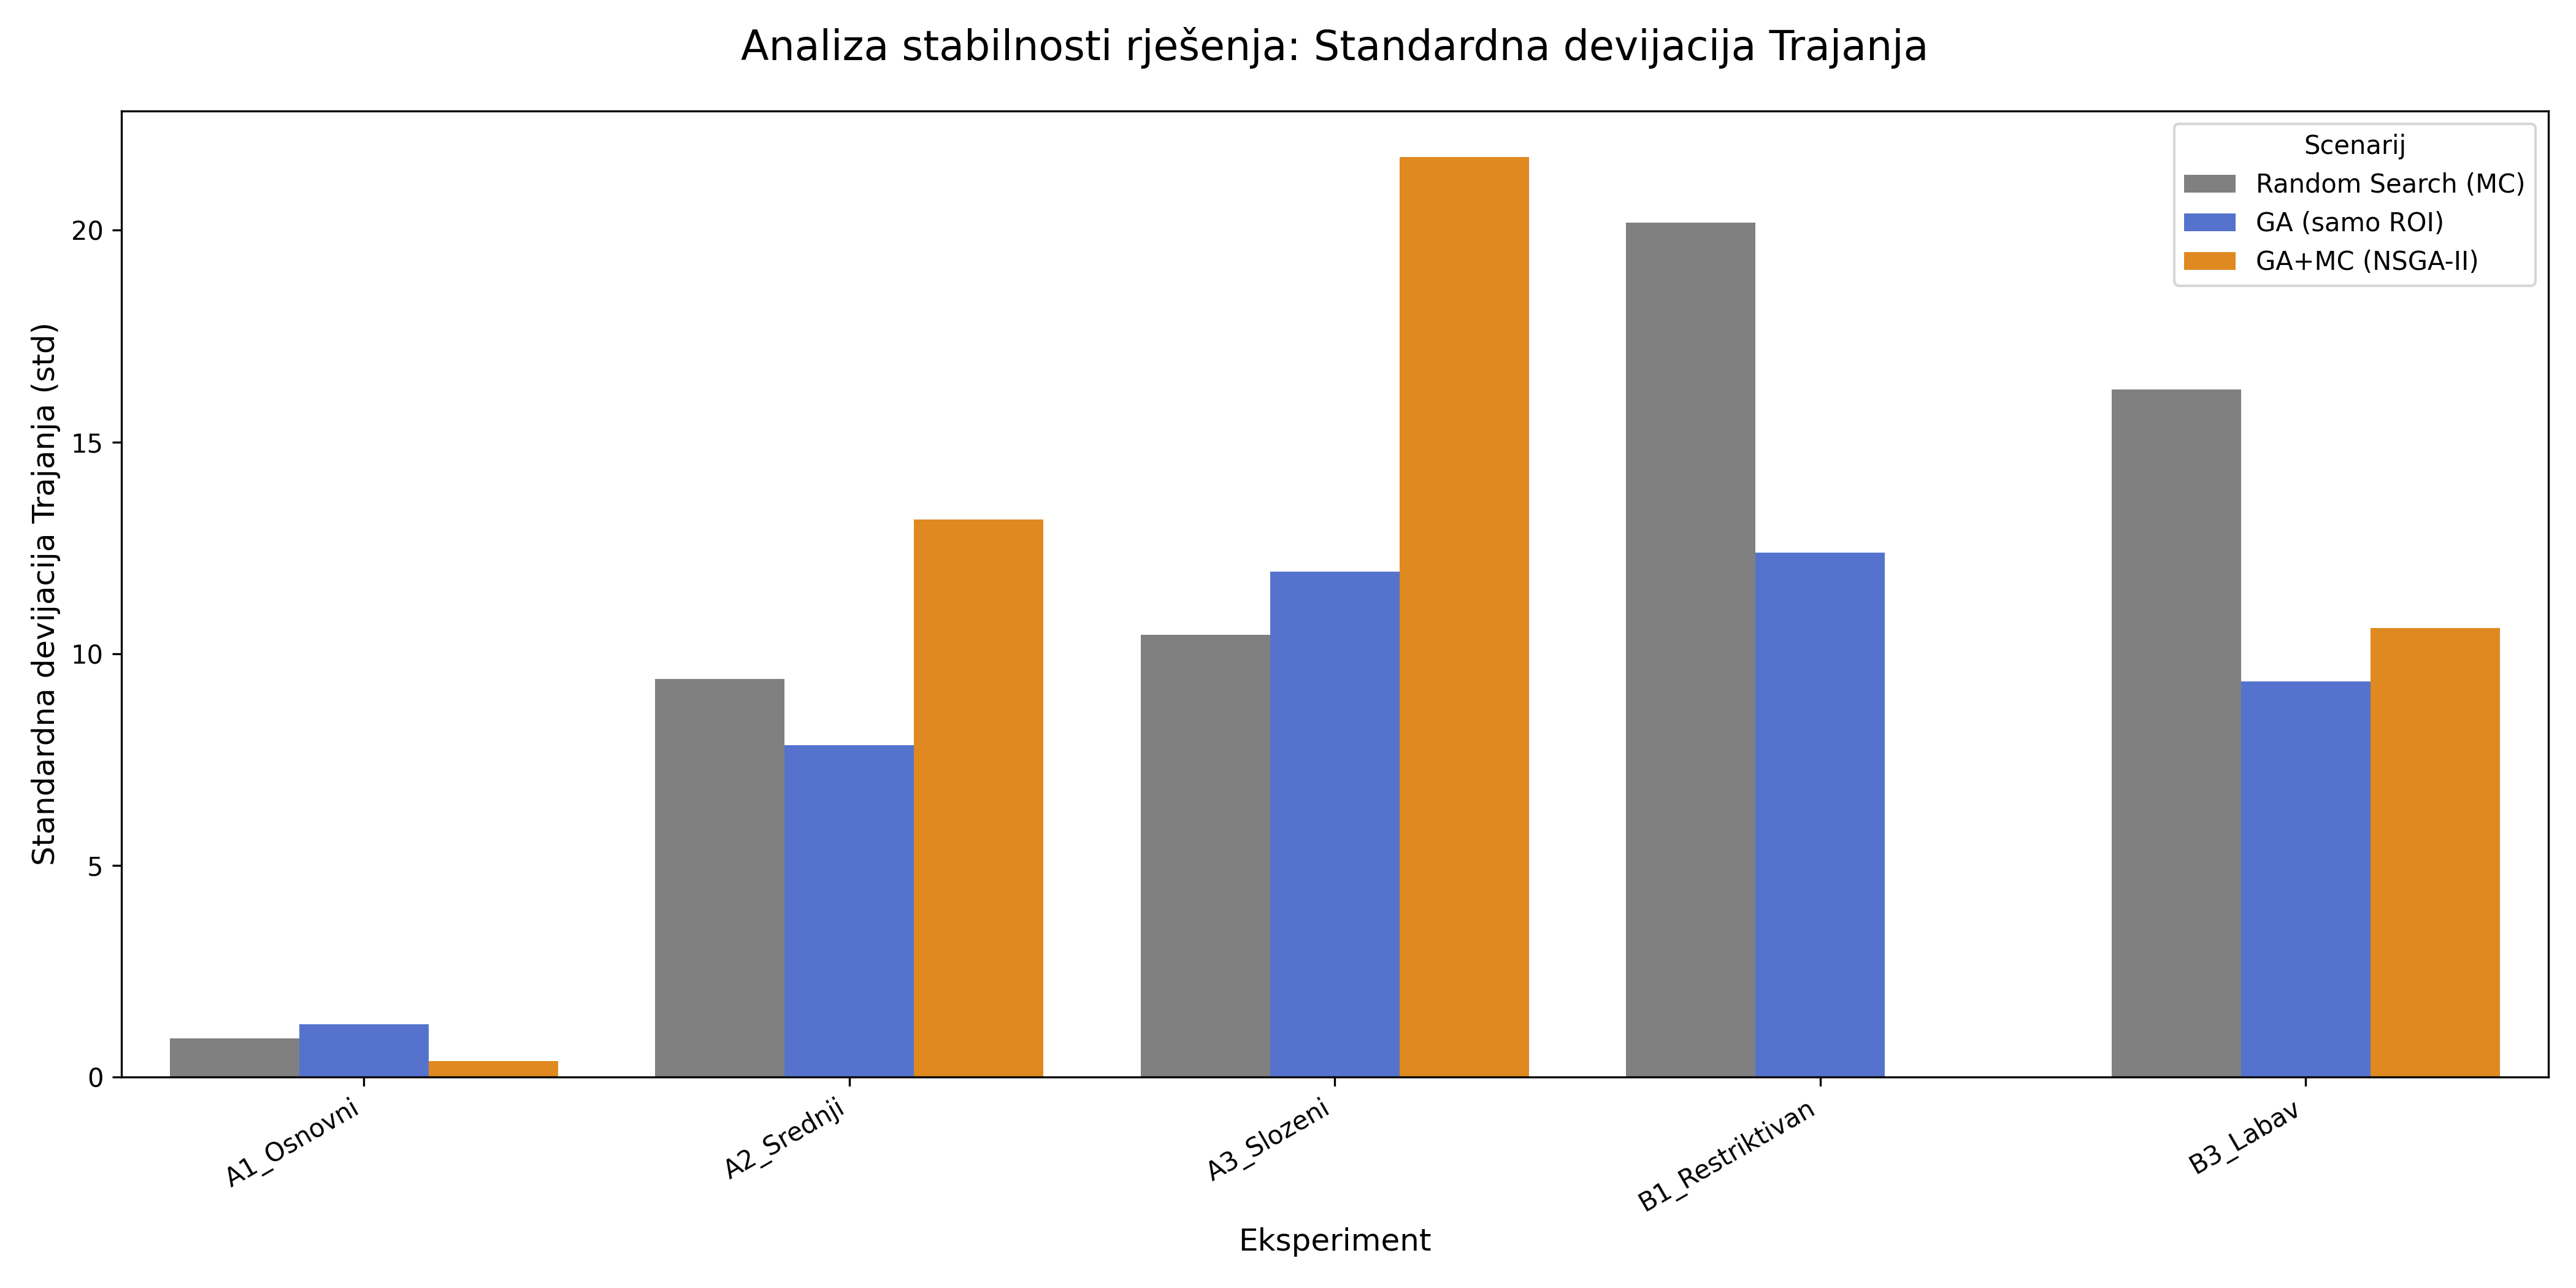
\includegraphics[width=\textwidth]{slike/grafikoni_final/C_stabilnost_trajanje.png}
        \caption{Stabilnost trajanja.}
    \end{subfigure}
    \caption{Grafički prikaz stabilnosti rješenja: Standardna devijacija za ROI i Trajanje.}
    \label{fig:stabilnost}
\end{figure}

\textbf{Dubinska analiza kompromisa: Paretov front}
Raspršeni dijagram na Slici~\ref{fig:pareto_front} pruža dubinski uvid u srž više-kriterijske optimizacije. On prikazuje Paretov front dobiven iz jednog pokretanja GA+MC (NSGA-II) modela na najsloženijem problemu (A3). Svaka točka na grafikonu predstavlja jedno optimalno, ne-dominirano rješenje i ilustrira temeljni kompromis (\emph{trade-off}) između profitabilnosti (Y-os) i rizika trajanja (X-os). Paretov front stoga ne nudi jedno "točno" rješenje, već služi kao strateški alat za donošenje odluka.

\begin{figure}[H]
    \centering
    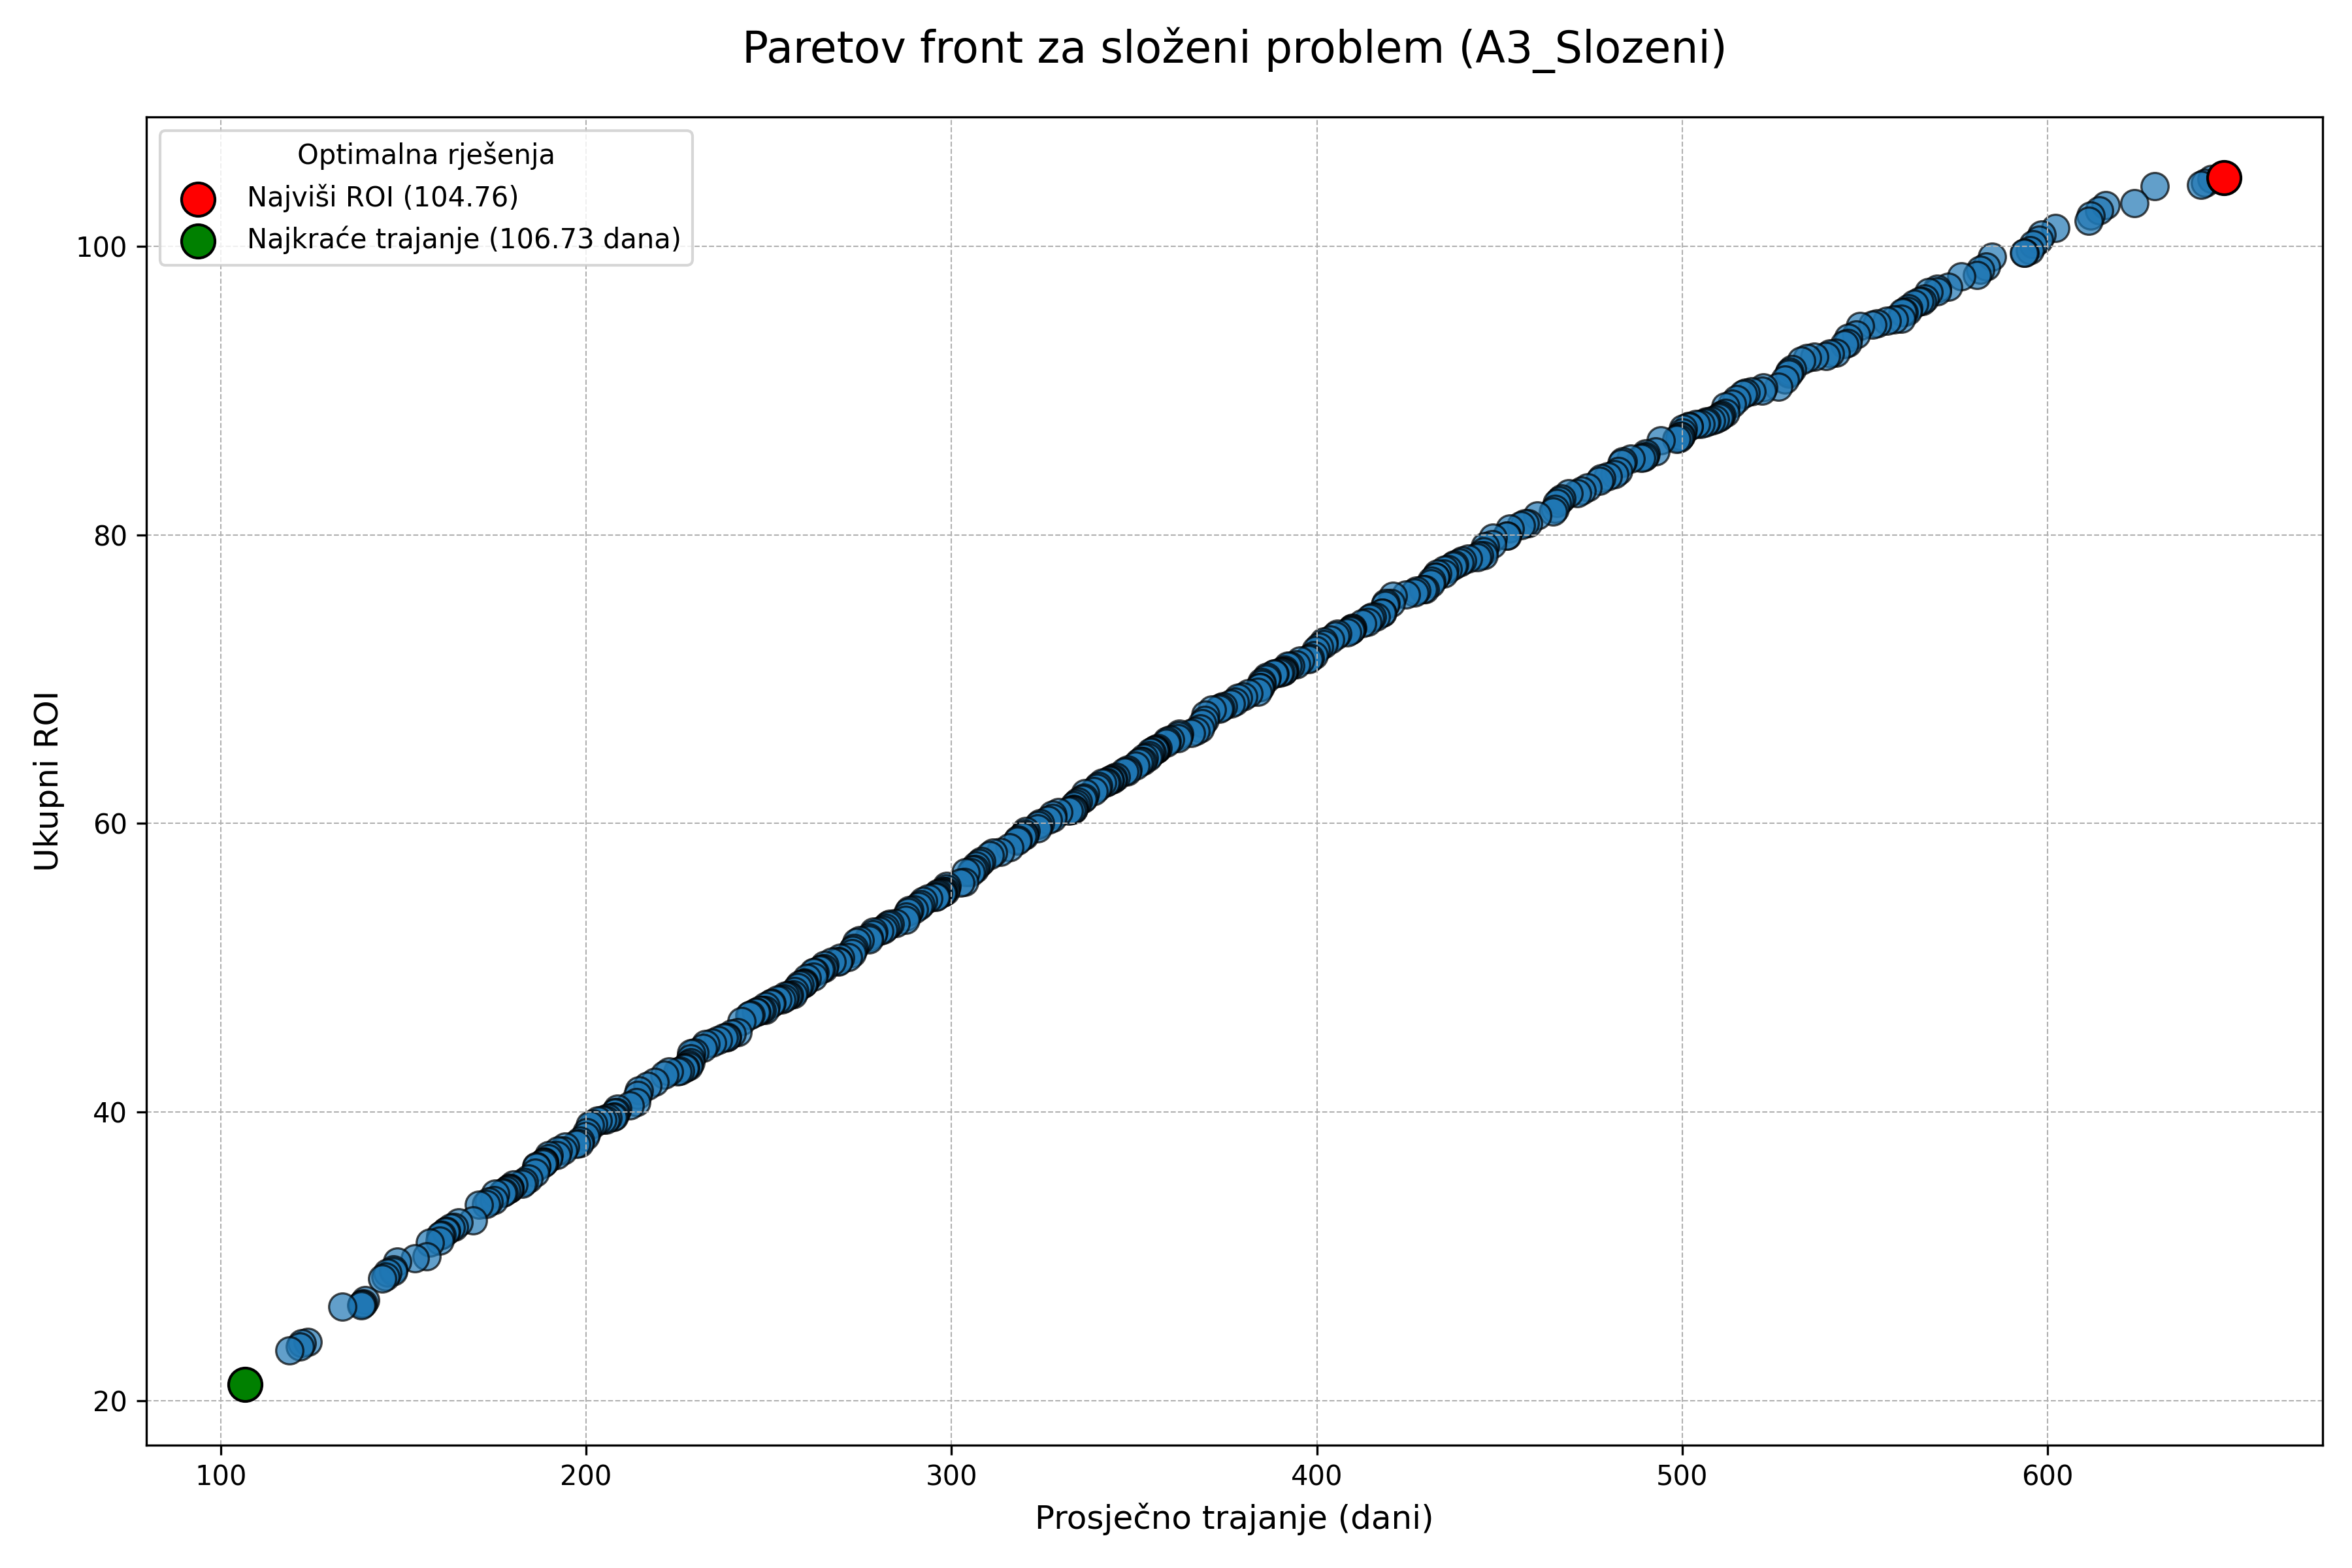
\includegraphics[width=0.9\textwidth]{slike/grafikoni_final/D_pareto_front_scatter.png}
    \caption{Paretov front za složeni problem (A3), koji prikazuje kompromis između ROI-a i trajanja.}
    \label{fig:pareto_front}
\end{figure}

\subsection{Sinteza glavnih zaključaka eksperimenata}
Provedeni eksperimenti omogućuju donošenje cjelovitih zaključaka o svakom modelu. Random Search (MC) se pokazao korisnim isključivo kao početna točka na jednostavnim problemima, ali je potpuno neadekvatan kao ozbiljan optimizacijski alat za probleme realne veličine. GA (samo ROI) je izuzetno snažan i robustan "profitni maksimizator", idealan u situacijama gdje je financijska dobit jedini kriterij. Konačno, GA+MC (NSGA-II) je sofisticirani "upravitelj rizikom", čija najveća vrijednost leži u pružanju strateških opcija koje balansiraju profit i rizik. Iako je superioran u standardnim i složenim uvjetima, njegova složenost ga čini osjetljivim u okruženjima s ekstremno restriktivnim ograničenjima.

Konačan izbor modela stoga ovisi o strateškim prioritetima projektnog ureda. Za maksimalan profit, klasični GA je pobjednik. Za uravnoteženo i rizikom informirano donošenje odluka, hibridni GA+MC je superioran, uz nužan oprez pri primjeni u vrlo ograničenim uvjetima.
